\documentclass[11pt]{article}
\usepackage[utf8]{inputenc}
\usepackage{amsmath}
\usepackage{amsfonts}
\usepackage{amssymb}
\usepackage{geometry}
\usepackage{enumitem}
\usepackage{graphicx}
\usepackage{tikz}
\usepackage{pgfplots}
\usepackage{amsthm}
\usepackage{mathtools}
\usepackage{tikz-cd}
\usepackage{hyperref}

\geometry{margin=1in}

\newtheorem{definition}{Definition}[section]
\newtheorem{theorem}{Theorem}[section]
\newtheorem{lemma}{Lemma}[section]
\newtheorem{corollary}{Corollary}[section]
\newtheorem{example}{Example}[section]
\newtheorem{proposition}{Proposition}[section]
\newtheorem{conjecture}{Conjecture}[section]

\title{Compiler Design and Optimization}
\author{Mathematical Notes}
\date{\today}

\begin{document}

\maketitle
\tableofcontents
\newpage

\section{Introduction to Compilers}

\subsection{What is a Compiler?}

\begin{definition}[Compiler]
A compiler is a computer program that translates source code written in a high-level programming language into target code (usually machine code or bytecode) that can be executed by a computer.
\end{definition}

The compilation process typically involves several phases:
\begin{enumerate}
    \item \textbf{Lexical Analysis} - Breaking source code into tokens
    \item \textbf{Syntax Analysis} - Parsing tokens into abstract syntax trees
    \item \textbf{Semantic Analysis} - Type checking and semantic validation
    \item \textbf{Intermediate Code Generation} - Creating intermediate representation
    \item \textbf{Code Optimization} - Improving the intermediate code
    \item \textbf{Code Generation} - Producing target machine code
\end{enumerate}

\subsection{Compiler Architecture}

Modern compilers typically follow a multi-pass architecture:

\begin{center}
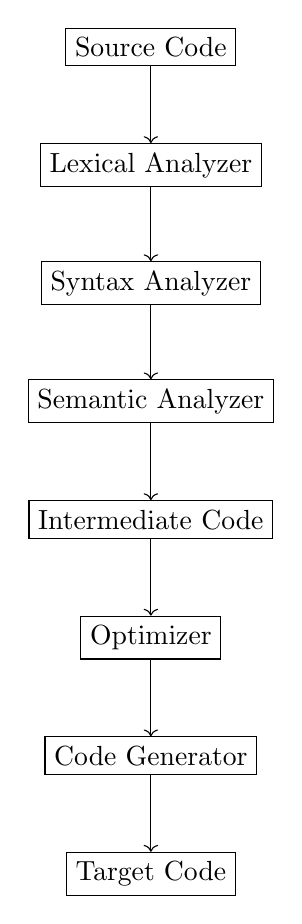
\begin{tikzpicture}[node distance=1.5cm]
    \node (source) [rectangle, draw] {Source Code};
    \node (lexer) [rectangle, draw, below of=source] {Lexical Analyzer};
    \node (parser) [rectangle, draw, below of=lexer] {Syntax Analyzer};
    \node (semantic) [rectangle, draw, below of=parser] {Semantic Analyzer};
    \node (ir) [rectangle, draw, below of=semantic] {Intermediate Code};
    \node (opt) [rectangle, draw, below of=ir] {Optimizer};
    \node (codegen) [rectangle, draw, below of=opt] {Code Generator};
    \node (target) [rectangle, draw, below of=codegen] {Target Code};
    
    \draw [->] (source) -- (lexer);
    \draw [->] (lexer) -- (parser);
    \draw [->] (parser) -- (semantic);
    \draw [->] (semantic) -- (ir);
    \draw [->] (ir) -- (opt);
    \draw [->] (opt) -- (codegen);
    \draw [->] (codegen) -- (target);
\end{tikzpicture}
\end{center}

\section{Lexical Analysis}

\subsection{Regular Expressions and Finite Automata}

\begin{definition}[Regular Expression]
A regular expression over alphabet $\Sigma$ is defined recursively:
\begin{itemize}
    \item $\emptyset$ (empty set)
    \item $\varepsilon$ (empty string)
    \item $a$ for $a \in \Sigma$
    \item $r_1 + r_2$ (union)
    \item $r_1 \cdot r_2$ (concatenation)
    \item $r^*$ (Kleene star)
\end{itemize}
\end{definition}

\begin{theorem}[Kleene's Theorem]
A language is regular if and only if it can be described by a regular expression.
\end{theorem}

\subsection{Finite State Automata}

\begin{definition}[Deterministic Finite Automaton (DFA)]
A DFA is a 5-tuple $M = (Q, \Sigma, \delta, q_0, F)$ where:
\begin{itemize}
    \item $Q$ is a finite set of states
    \item $\Sigma$ is the input alphabet
    \item $\delta: Q \times \Sigma \to Q$ is the transition function
    \item $q_0 \in Q$ is the start state
    \item $F \subseteq Q$ is the set of accepting states
\end{itemize}
\end{definition}

\begin{definition}[Non-deterministic Finite Automaton (NFA)]
An NFA is a 5-tuple $M = (Q, \Sigma, \delta, q_0, F)$ where:
\begin{itemize}
    \item $Q$ is a finite set of states
    \item $\Sigma$ is the input alphabet
    \item $\delta: Q \times (\Sigma \cup \{\varepsilon\}) \to 2^Q$ is the transition function
    \item $q_0 \in Q$ is the start state
    \item $F \subseteq Q$ is the set of accepting states
\end{itemize}
\end{definition}

\subsection{Lexical Analysis Implementation}

The lexical analyzer (lexer) converts a stream of characters into a stream of tokens. Common token types include:
\begin{itemize}
    \item Keywords (if, while, class, etc.)
    \item Identifiers (variable names)
    \item Literals (numbers, strings)
    \item Operators (+, -, *, /, etc.)
    \item Delimiters (parentheses, semicolons, etc.)
\end{itemize}

\section{Syntax Analysis}

\subsection{Context-Free Grammars}

\begin{definition}[Context-Free Grammar]
A context-free grammar is a 4-tuple $G = (V, T, P, S)$ where:
\begin{itemize}
    \item $V$ is a finite set of non-terminals
    \item $T$ is a finite set of terminals
    \item $P$ is a finite set of productions of the form $A \to \alpha$
    \item $S \in V$ is the start symbol
\end{itemize}
\end{definition}

\begin{example}[Simple Arithmetic Grammar]
\begin{align}
E &\to E + T \mid T \\
T &\to T * F \mid F \\
F &\to (E) \mid \text{id}
\end{align}
\end{example}

\subsection{Parsing Algorithms}

\subsubsection{Top-Down Parsing}

\begin{definition}[LL(k) Grammar]
A grammar is LL(k) if it can be parsed deterministically from left to right, producing a leftmost derivation, using k tokens of lookahead.
\end{definition}

\textbf{Recursive Descent Parsing:}
\begin{itemize}
    \item Each non-terminal corresponds to a procedure
    \item Procedure bodies implement the grammar rules
    \item Requires LL(1) grammar for deterministic parsing
\end{itemize}

\textbf{Predictive Parsing:}
\begin{itemize}
    \item Uses parsing table to make decisions
    \item Constructs FIRST and FOLLOW sets
    \item Eliminates left recursion and left factoring
\end{itemize}

\subsubsection{Bottom-Up Parsing}

\begin{definition}[LR(k) Grammar]
A grammar is LR(k) if it can be parsed deterministically from left to right, producing a rightmost derivation in reverse, using k tokens of lookahead.
\end{definition}

\textbf{LR(1) Parsing:}
\begin{itemize}
    \item Uses canonical LR(1) items
    \item Constructs parsing table with ACTION and GOTO
    \item Handles reduce-reduce and shift-reduce conflicts
\end{itemize}

\textbf{LALR(1) Parsing:}
\begin{itemize}
    \item Merges LR(1) states with same core
    \item Smaller parsing tables than LR(1)
    \item May introduce reduce-reduce conflicts
\end{itemize}

\subsection{Abstract Syntax Trees}

\begin{definition}[Abstract Syntax Tree (AST)]
An AST is a tree representation of the syntactic structure of source code, where each node represents a construct occurring in the source code.
\end{definition}

The AST abstracts away from the concrete syntax and focuses on the essential structure of the program.

\section{Semantic Analysis}

\subsection{Type Systems}

\begin{definition}[Type System]
A type system is a tractable syntactic method for proving the absence of certain program behaviors by classifying phrases according to the kinds of values they compute.
\end{definition}

\subsubsection{Type Checking}

\textbf{Static Type Checking:}
\begin{itemize}
    \item Performed at compile time
    \item Catches type errors before execution
    \item Requires type annotations or type inference
\end{itemize}

\textbf{Dynamic Type Checking:}
\begin{itemize}
    \item Performed at runtime
    \item More flexible but less efficient
    \item Runtime type errors possible
\end{itemize}

\subsubsection{Type Inference}

\begin{definition}[Type Inference]
Type inference is the process of automatically determining the types of expressions in a program without explicit type annotations.
\end{definition}

\textbf{Hindley-Milner Type System:}
\begin{itemize}
    \item Polymorphic type system
    \item Algorithm W for type inference
    \item Unification-based approach
\end{itemize}

\subsection{Symbol Tables}

\begin{definition}[Symbol Table]
A symbol table is a data structure used by a compiler to keep track of semantic information about various source language constructs.
\end{definition}

Symbol tables typically store:
\begin{itemize}
    \item Variable names and types
    \item Function signatures
    \item Class definitions
    \item Scope information
\end{itemize}

\section{Intermediate Code Generation}

\subsection{Intermediate Representations}

\subsubsection{Three-Address Code}

\begin{definition}[Three-Address Code]
Three-address code is an intermediate representation where each instruction has at most one operator and three operands.
\end{definition}

\begin{example}[Three-Address Code]
\begin{align}
t_1 &= a + b \\
t_2 &= t_1 * c \\
d &= t_2
\end{align}
\end{example}

\subsubsection{Static Single Assignment (SSA)}

\begin{definition}[Static Single Assignment]
In SSA form, each variable is assigned exactly once, and every use of a variable is dominated by its definition.
\end{definition}

SSA form enables:
\begin{itemize}
    \item Efficient data-flow analysis
    \item Dead code elimination
    \item Constant propagation
    \item Register allocation
\end{itemize}

\subsection{Control Flow Graphs}

\begin{definition}[Control Flow Graph]
A control flow graph (CFG) is a directed graph where nodes represent basic blocks and edges represent control flow between blocks.
\end{definition}

\begin{definition}[Basic Block]
A basic block is a sequence of consecutive statements with a single entry point and a single exit point.
\end{definition}

\section{Code Optimization}

\subsection{Optimization Levels}

\begin{enumerate}
    \item \textbf{Local Optimization} - Within basic blocks
    \item \textbf{Global Optimization} - Across basic blocks
    \item \textbf{Interprocedural Optimization} - Across procedure boundaries
\end{enumerate}

\subsection{Data-Flow Analysis}

\begin{definition}[Data-Flow Analysis]
Data-flow analysis is a technique for gathering information about the possible set of values calculated at various points in a computer program.
\end{definition}

\subsubsection{Reaching Definitions}

\begin{definition}[Reaching Definition]
A definition $d$ reaches a point $p$ if there exists a path from $d$ to $p$ such that $d$ is not killed along that path.
\end{definition}

The reaching definitions problem can be formulated as:
\begin{align}
\text{REACH}[n] &= \text{GEN}[n] \cup (\text{REACH}[m] - \text{KILL}[n])
\end{align}
where $m$ is a predecessor of $n$.

\subsubsection{Live Variables}

\begin{definition}[Live Variable]
A variable $v$ is live at a point $p$ if there exists a path from $p$ to a use of $v$ that does not redefine $v$.
\end{definition}

\subsection{Optimization Techniques}

\subsubsection{Constant Folding and Propagation}

\begin{definition}[Constant Folding]
Constant folding is the process of evaluating constant expressions at compile time.
\end{definition}

\begin{definition}[Constant Propagation]
Constant propagation is the process of replacing variables with their constant values when possible.
\end{definition}

\subsubsection{Dead Code Elimination}

\begin{definition}[Dead Code]
Dead code is code that can never be executed or whose results are never used.
\end{definition}

Dead code elimination removes:
\begin{itemize}
    \item Unreachable code
    \item Unused variables
    \item Unused functions
\end{itemize}

\subsubsection{Common Subexpression Elimination}

\begin{definition}[Common Subexpression Elimination]
CSE identifies and eliminates redundant computations of the same expression.
\end{definition}

\subsubsection{Loop Optimizations}

\textbf{Loop Invariant Code Motion:}
\begin{itemize}
    \item Moves computations outside loops
    \item Reduces redundant calculations
\end{itemize}

\textbf{Loop Unrolling:}
\begin{itemize}
    \item Replicates loop body multiple times
    \item Reduces loop overhead
    \item Enables further optimizations
\end{itemize}

\textbf{Induction Variable Elimination:}
\begin{itemize}
    \item Eliminates unnecessary induction variables
    \item Simplifies loop conditions
\end{itemize}

\subsubsection{Function Inlining}

\begin{definition}[Function Inlining]
Function inlining replaces a function call with the body of the called function.
\end{definition}

Benefits:
\begin{itemize}
    \item Eliminates call overhead
    \item Enables further optimizations
    \item May increase code size
\end{itemize}

\section{Register Allocation}

\subsection{Graph Coloring}

\begin{definition}[Register Allocation]
Register allocation is the process of assigning program variables to processor registers.
\end{definition}

\begin{theorem}[Graph Coloring Theorem]
A graph is $k$-colorable if and only if it does not contain a complete subgraph of size $k+1$.
\end{theorem}

\subsection{Interference Graphs}

\begin{definition}[Interference Graph]
An interference graph is a graph where nodes represent variables and edges represent variables that cannot be assigned to the same register.
\end{definition}

\textbf{Chaitin's Algorithm:}
\begin{enumerate}
    \item Build interference graph
    \item Simplify graph by removing low-degree nodes
    \item Spill nodes if graph is not colorable
    \item Color the graph
\end{enumerate}

\subsection{Spilling}

\begin{definition}[Spilling]
Spilling is the process of storing variables in memory when there are not enough registers.
\end{definition}

Spill heuristics:
\begin{itemize}
    \item Spill variables with high spill cost
    \item Spill variables with low usage frequency
    \item Consider loop nesting levels
\end{itemize}

\section{Code Generation}

\subsection{Instruction Selection}

\begin{definition}[Instruction Selection]
Instruction selection is the process of choosing appropriate machine instructions to implement each intermediate code operation.
\end{definition}

\textbf{Tree Pattern Matching:}
\begin{itemize}
    \item Represent instructions as tree patterns
    \item Use dynamic programming for optimal selection
    \item Handle complex addressing modes
\end{itemize}

\subsection{Instruction Scheduling}

\begin{definition}[Instruction Scheduling]
Instruction scheduling is the process of reordering instructions to improve performance while maintaining correctness.
\end{definition}

\textbf{Pipeline Scheduling:}
\begin{itemize}
    \item Minimize pipeline stalls
    \item Consider instruction latencies
    \item Handle data dependencies
\end{itemize}

\subsection{Peephole Optimization}

\begin{definition}[Peephole Optimization]
Peephole optimization is a local optimization technique that examines a small window of instructions and replaces them with more efficient sequences.
\end{definition}

Common peephole optimizations:
\begin{itemize}
    \item Redundant load elimination
    \item Strength reduction
    \item Branch optimization
\end{itemize}

\section{Advanced Topics}

\subsection{Just-In-Time Compilation}

\begin{definition}[Just-In-Time Compilation]
JIT compilation is a method of executing computer code that involves compilation during program execution rather than before.
\end{definition}

JIT compilation benefits:
\begin{itemize}
    \item Profile-guided optimization
    \item Adaptive optimization
    \item Runtime specialization
\end{itemize}

\subsection{Parallel Compilation}

\begin{definition}[Parallel Compilation]
Parallel compilation distributes compilation tasks across multiple processors to reduce compilation time.
\end{definition}

Parallelization strategies:
\begin{itemize}
    \item File-level parallelism
    \item Function-level parallelism
    \item Phase-level parallelism
\end{itemize}

\subsection{Compiler Correctness}

\begin{definition}[Compiler Correctness]
A compiler is correct if it preserves the semantics of the source program in the target program.
\end{definition}

Verification techniques:
\begin{itemize}
    \item Translation validation
    \item Formal verification
    \item Testing and validation
\end{itemize}

\section{Modern Compiler Design}

\subsection{Multi-Pass Architecture}

Modern compilers often use multiple passes for:
\begin{itemize}
    \item Modularity and maintainability
    \item Different optimization levels
    \item Language-specific processing
\end{itemize}

\subsection{Plugin Architecture}

\begin{definition}[Plugin Architecture]
A plugin architecture allows extending compiler functionality through dynamically loaded modules.
\end{definition}

Benefits:
\begin{itemize}
    \item Language-specific optimizations
    \item Target-specific code generation
    \item Custom analysis passes
\end{itemize}

\subsection{Compiler Infrastructure}

Popular compiler infrastructures:
\begin{itemize}
    \item \textbf{LLVM} - Low Level Virtual Machine
    \item \textbf{GCC} - GNU Compiler Collection
    \item \textbf{MLIR} - Multi-Level Intermediate Representation
\end{itemize}

\section{Performance Analysis}

\subsection{Compilation Metrics}

Key performance metrics:
\begin{itemize}
    \item Compilation time
    \item Memory usage
    \item Generated code size
    \item Runtime performance
\end{itemize}

\subsection{Optimization Effectiveness}

Measuring optimization effectiveness:
\begin{itemize}
    \item Benchmark suites
    \item Profiling tools
    \item Performance counters
\end{itemize}

\section{Conclusion}

Compiler design and optimization is a complex field that combines theoretical computer science with practical engineering. The key principles include:

\begin{itemize}
    \item Modular design with clear separation of concerns
    \item Systematic application of optimization techniques
    \item Careful balance between compilation time and code quality
    \item Adaptation to modern hardware architectures
\end{itemize}

The field continues to evolve with new languages, architectures, and optimization techniques, making it an exciting area of computer science research and development.

\end{document}
